\documentclass[../Supercritical_fluid_extraction_of_essential_oil_from_chamomile.tex]{subfiles}
\graphicspath{{\subfix{../Figures/}}}
\begin{document}
	
	\label{CH: Results}
	
	To solve the parameter estimation problem, the single shooting method was used to transform the boundary-value problem into the initial value problem and to formulate the non-linear programming problem. This non-linear optimization task was tackled using the CasADi framework (\citet{Andersson2018}). Each time series was fitted separately to the model with the linear extraction kinetics (Equation \ref{Model_kinetic_no_sat}). The initial value problem was solved multiple times with varying initial guesses to identify the global minimum. Within the model context characterized by linear kinetics, two parameters remain to be determined: the partition coefficient $k_m$ and the internal diffusion coefficient $D_i$. 
	
	\begin{figure}[!h]
		\centering
		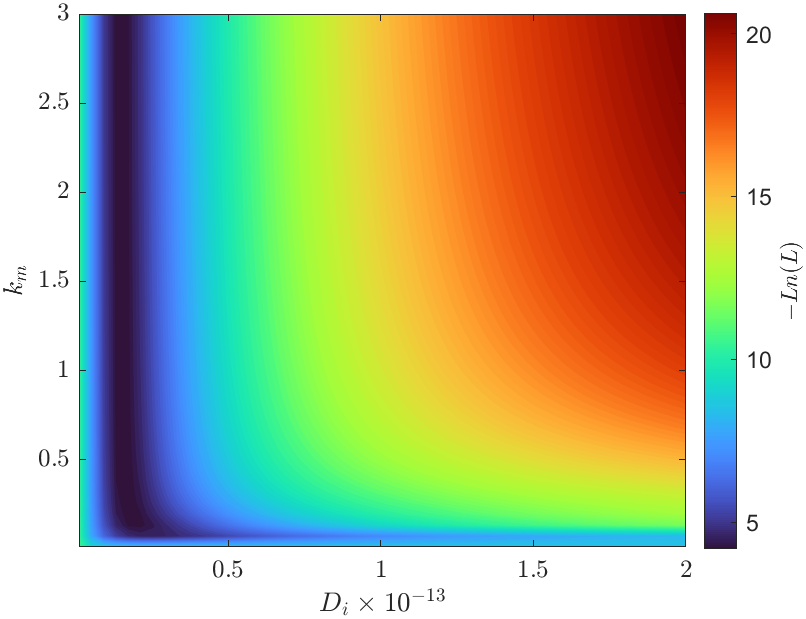
\includegraphics[trim = 0.0cm 0.0cm 0.0cm 0.0cm,clip, width=\columnwidth]{/Results_estimation/Parameter_Space_Linear_Dataset_1.png}
		\caption{Parameter space for the linear extraction kinetic model and the experiment 1}
		\label{fig: Fit_1_linear}
	\end{figure}
	
	Figure \ref{fig: Fit_1_linear} shows the parameter space and corresponding values of the cost function for experiment 1 ($40^\circ C$, 100 bar and 6.67$\times 10^{-5}$ kg/s). As the cost function is to be minimized, the lowest value of $-\ln(L)$ indicate the best fit. A black vertical stripe at $D_i \approx 0.2$ can be observed. That stripe indicates the existence of the optimal value of the $D_i$. In the direction of $k_m$, the cost function is almost flat, which suggests that any value of $k_m$ above 0.1 fits the data equally well. If $k_m$ can be an arbitrary point, then it can grow to infinity, which suggests that the solvent is far from the saturation, and the model can be simplified. The model reduction can be introduced by considering the limit of $k_m$ in the extraction kinetic term: 
	
	{\footnotesize
		\begin{equation*}
			\begin{split}
				&\lim_{k_m \rightarrow \infty} \left({\color{black}{\color{black} c_s} }(t,z)  - \cfrac{{\color{black}\rho_s}}{{\color{black}k_m}({\color{black}T}(t,z)){\color{black}\rho}({\color{black}T}(t,z),{\color{black}P}(t))}  {\color{black}c_f}(t,z) \right)  = \\
				&= \left({\color{black}{\color{black} c_s} }(t,z)  - \cfrac{\rho_s}{\infty \cdot \rho(T(t,z),P(t))}  {c_f}(t,z) \right) = \left(c_s(t,z) - 0 \right)
			\end{split}
	\end{equation*} }
	
	The extraction model can be adapted to incorporate adjustments for the reduced kinetic term and axial diffusion. In this revised setup, two parameters remain undetermined: the internal diffusion coefficient $D_i$ and the axial diffusion coefficient $D_e^M$. Figure \ref{fig: Fit_1_Di_Dx} illustrates the parameter space and associated cost function values.
	
	\begin{figure}[!h]
		\centering
		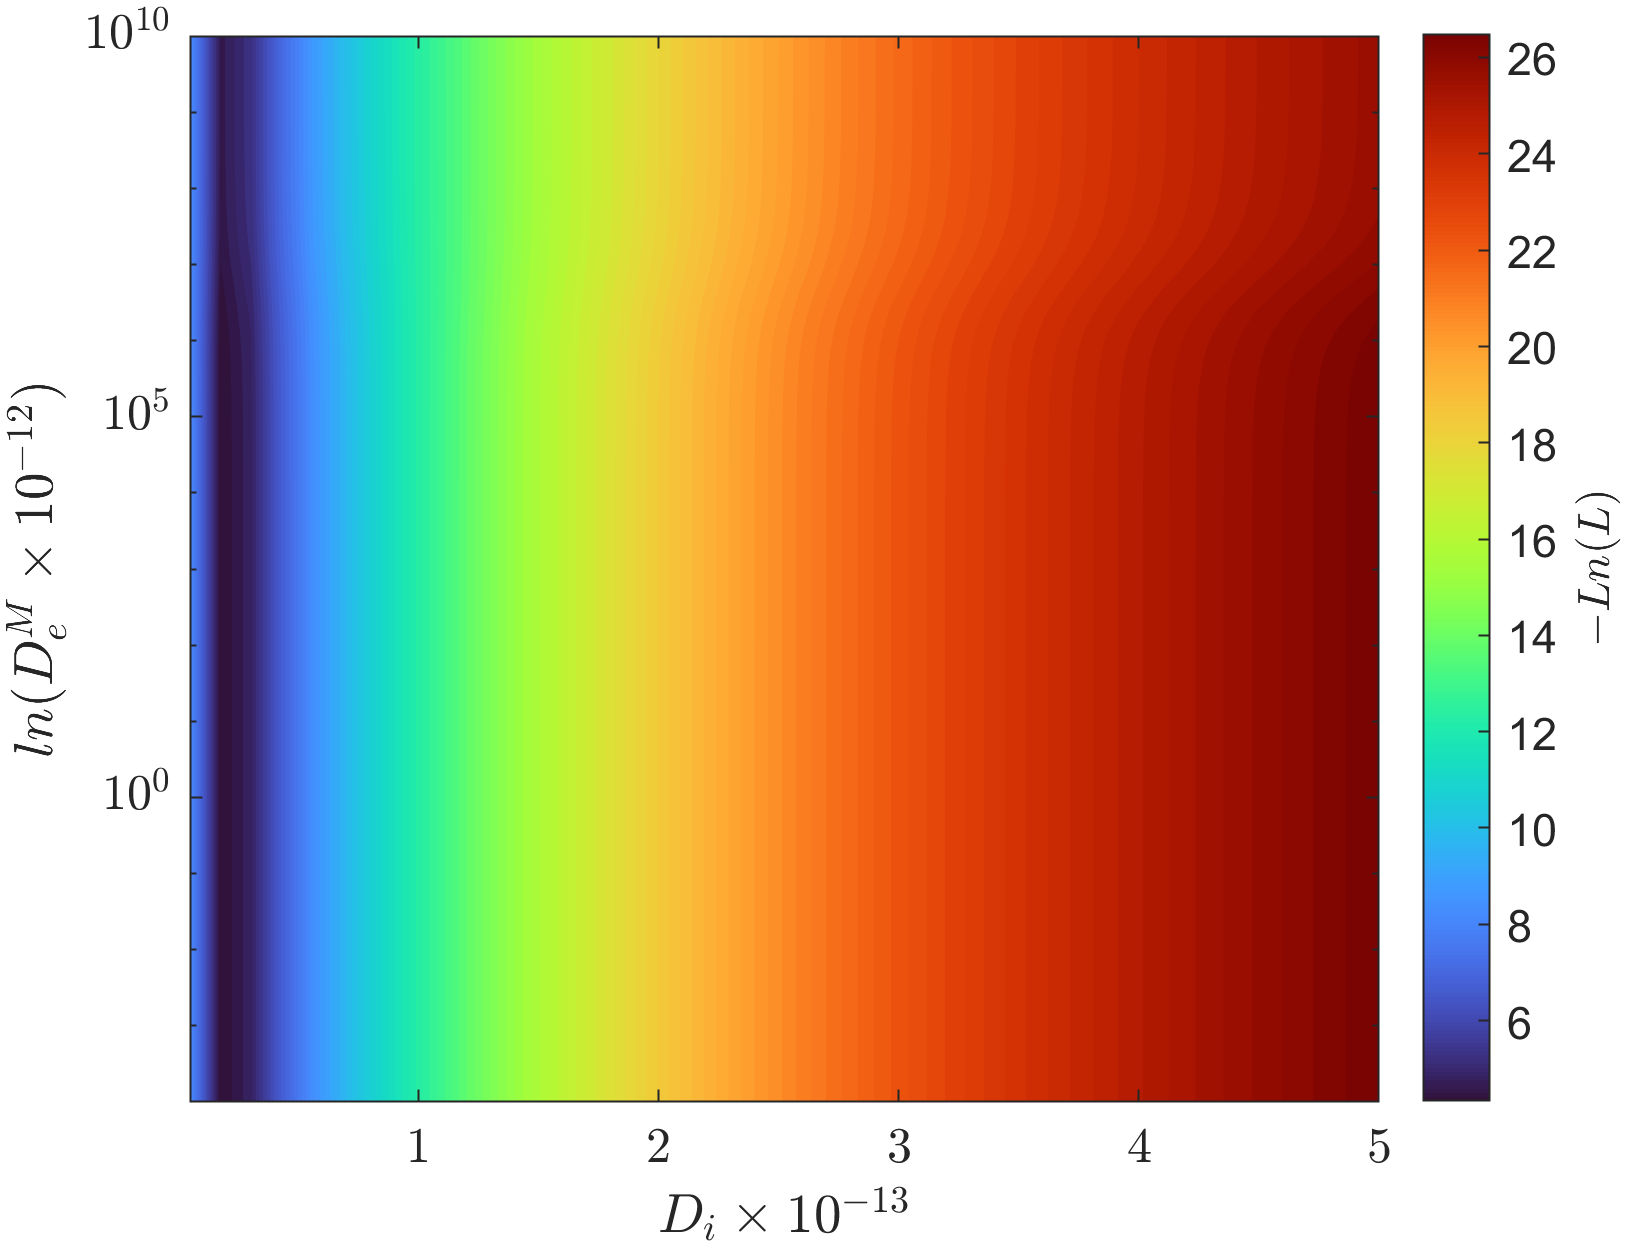
\includegraphics[trim = 0.0cm 0.0cm 0.0cm 0.0cm,clip, width=\columnwidth]{/Results_estimation/Parameter_Space_Di_Dx_Dataset_1.png}
		\caption{Parameter space for the reduced linear extraction kinetic model with and the experiment 1}
		\label{fig: Fit_1_Di_Dx}
	\end{figure}
	
	Similarly to the previous case, the optimal value of $D_i$ exists, but a unique value for the $D_e^M$ cannot be determined. Figure \ref{fig: Fit_1_Di_Dx} illustrates the minimal impact of the axial diffusion coefficient, where a broad range of $D_e^M$ yields identical cost function values. By selecting a low value $D_e^M$, the axial diffusion terms can be reduced or eliminated from the model without compromising its generality. This observation aligns with the findings of \citet{Rahimi2011}, who analysed the same dataset and reported Peclet numbers ranging between 290 and 400. Such high values of the Peclet number suggest that the advection term dominates the mass transfer, and the axial diffusion is negligible.
	
	In both scenarios previously discussed, the fitting outcomes were not deemed satisfactory. Building upon the concepts underlying the Broken-and-Intact and Shrinking Core models (detailed in Chapter \ref{CH: Gamma_Function}), a gamma function is introduced to capture the diminishing extraction kinetics. The correction factor is combined with the simplified linear model, resulting in a two-parameter model ($D_i^R$ and $\Upsilon$) as given by Equation \ref{Model_kinetic}. Figure \ref{fig: Fit_1_Di_Gamma} shows the parameter space and the corresponding cost function values.
	
	\begin{figure}[!h]
		\centering
		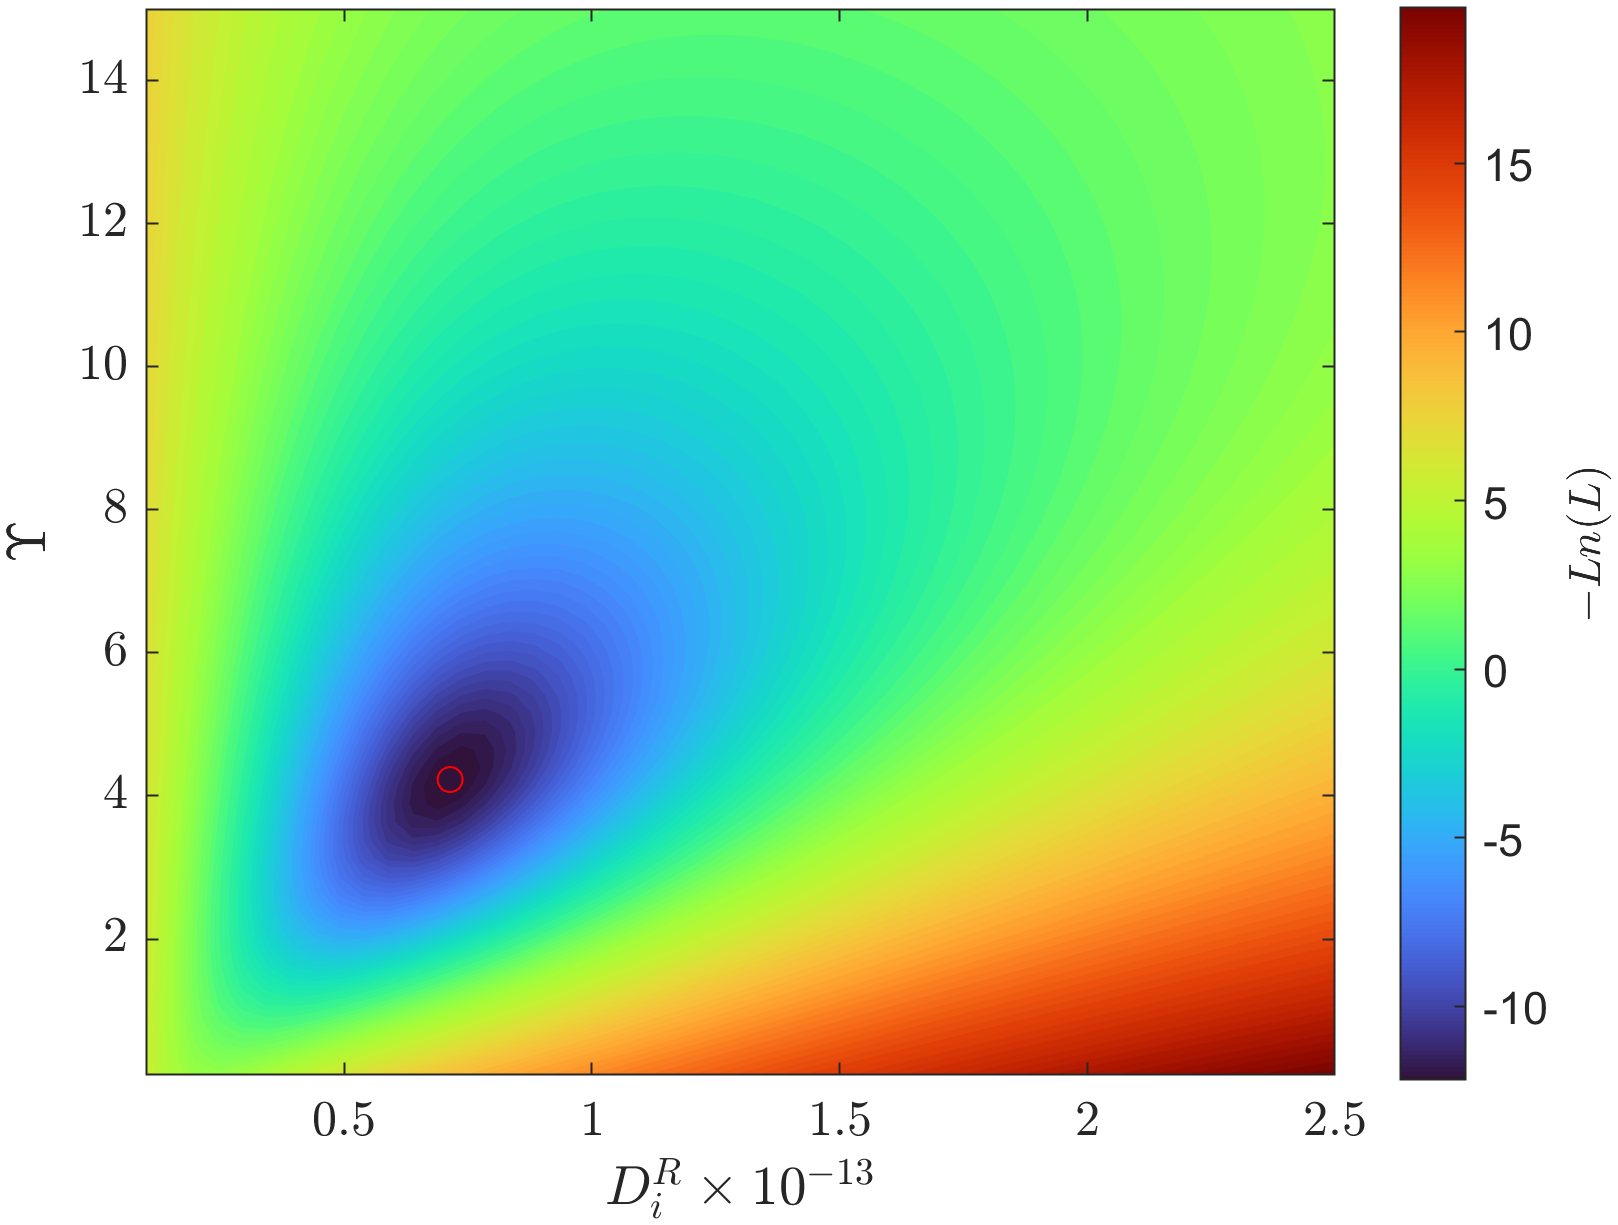
\includegraphics[trim = 0.0cm 0.0cm 0.0cm 0.0cm,clip, width=0.98\columnwidth]{/Results_estimation/Parameter_space_Di_Gamma_dataset_1_org.png}
		\caption{Parameter space for the modified extraction model and experiment 1}
		\label{fig: Fit_1_Di_Gamma}
	\end{figure}
	
	The parameter space for the revised model exhibits a distinct minimum value corresponding to the solution of the parameter estimation problem for experiment 1. The red circle highlights the minimum value of the cost function found by the optimizer. The remaining experiments are fitted to the modified extraction model, and results are presented in Figure \ref{fig: Fit_Di_Gamma}. The obtained results show good agreement with experimental data. 

	\begin{figure}[!h]
		\centering
		\begin{subfigure}[b]{\columnwidth}
			\centering
			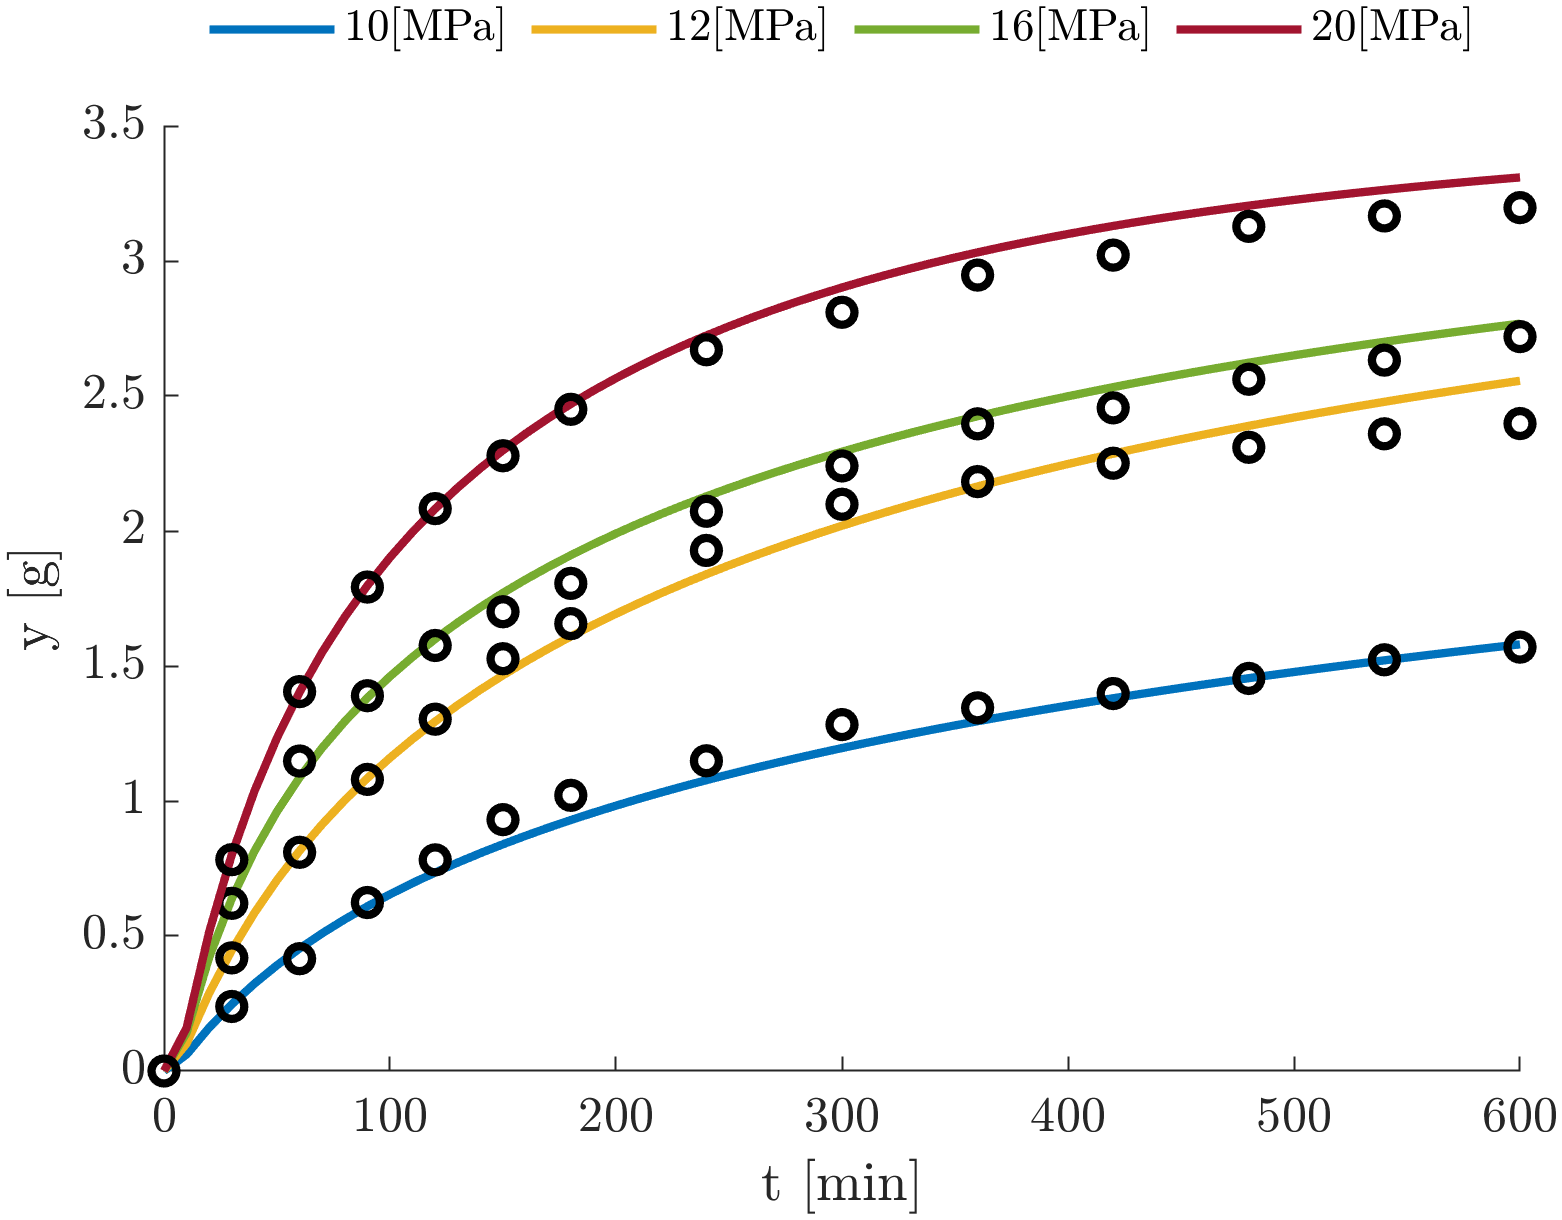
\includegraphics[trim = 0.0cm 0.0cm 0.0cm 0.0cm,clip, width=\columnwidth]{/Results_estimation/Fit_Di_Gamma_1_4.png}
			\caption{Results of parameter estimation for experiments at $6.67\times 10^{-5}$ [kg/s] and temperature of 40 $[^\circ C]$}
			\label{fig: Fit_1_4_Di_Gamma}
		\end{subfigure}
		\hfill
		\begin{subfigure}[b]{\columnwidth}
			\centering
			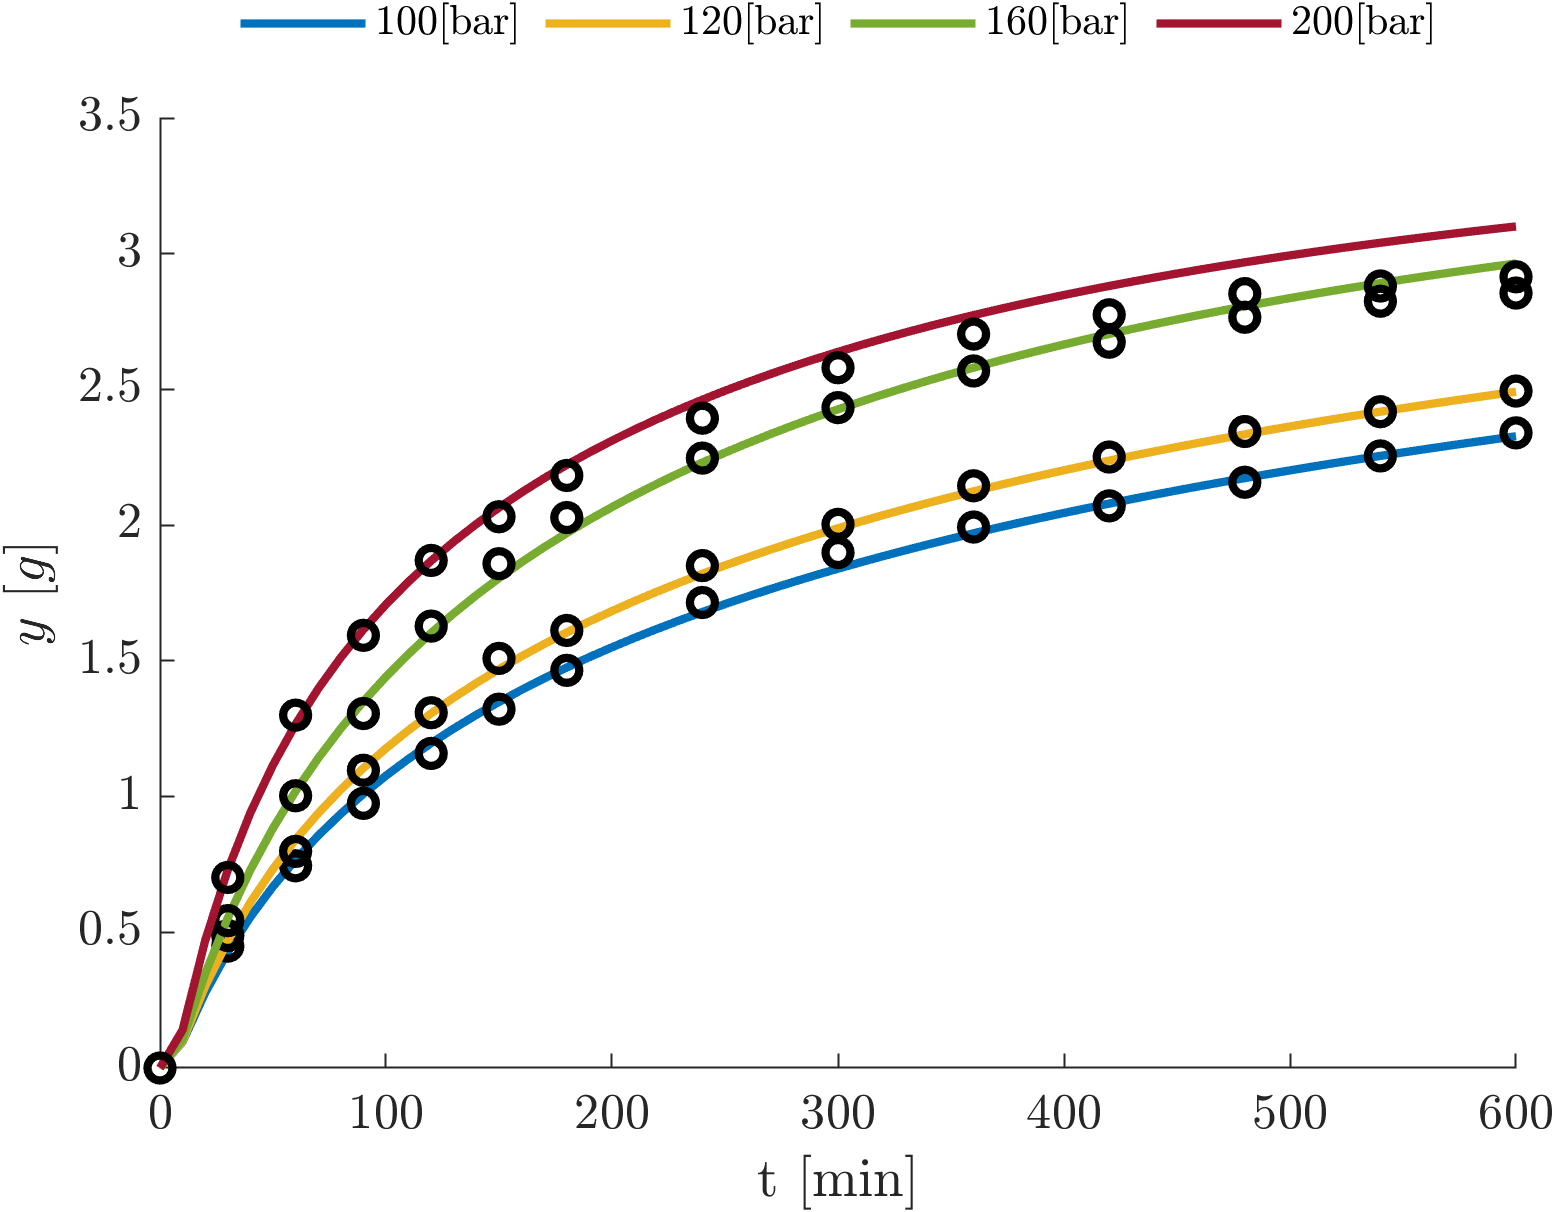
\includegraphics[trim = 0.0cm 0.0cm 0.0cm 0.0cm,clip, width=\columnwidth]{/Results_estimation/Fit_Di_Gamma_5_8.png}
			\caption{Results of parameter estimation for experiments at $6.67\times 10^{-5}$ [kg/s] and temperature of 30 $[^\circ C]$}
			\label{fig: Fit_5_8_Di_Gamma}
		\end{subfigure}
			\end{figure}%
		\begin{figure}[h!]\ContinuedFloat
		\begin{subfigure}[b]{\columnwidth}
			\centering
			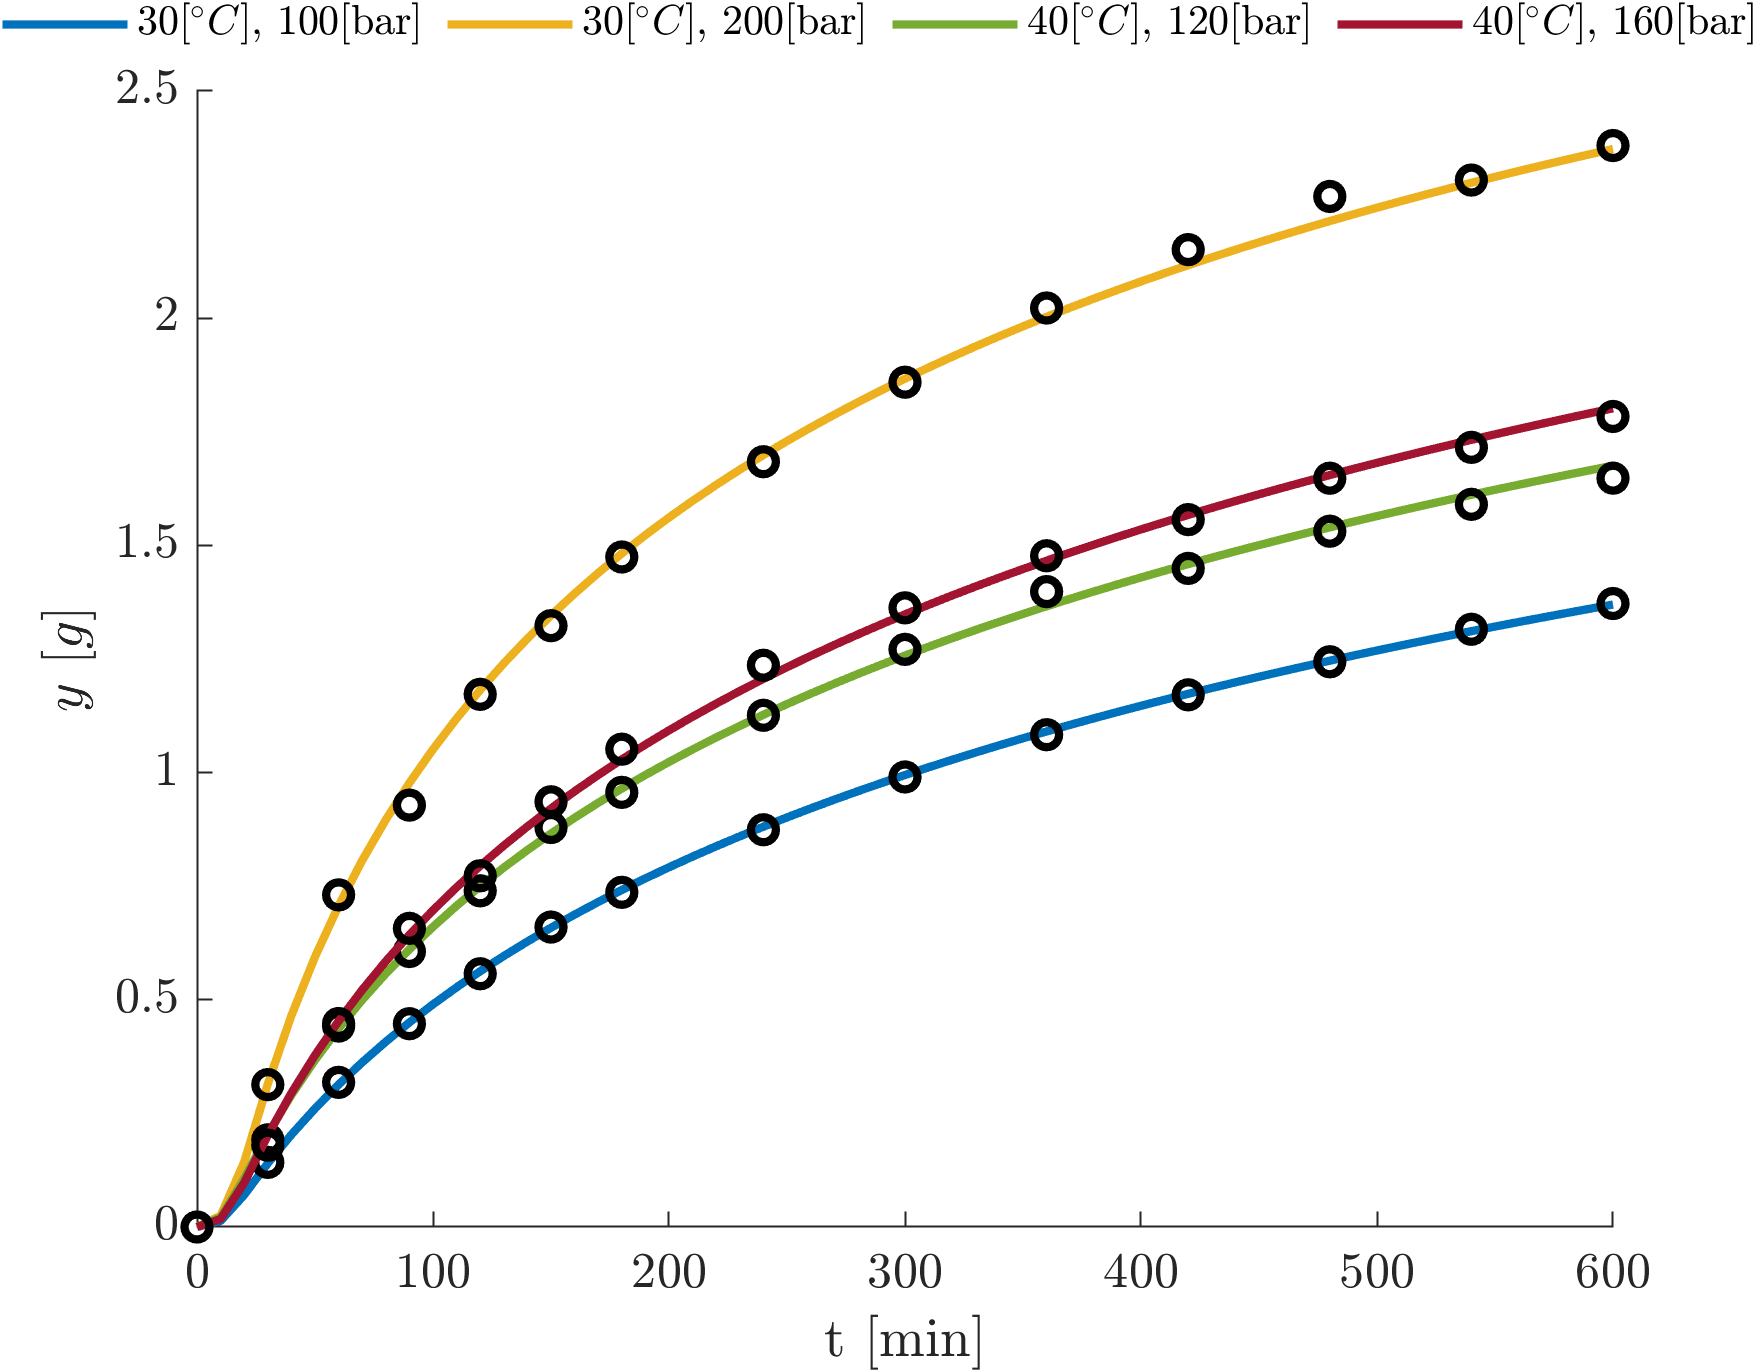
\includegraphics[trim = 0.0cm 0.0cm 0.0cm 0.0cm,clip, width=\columnwidth]{/Results_estimation/Fit_Di_Gamma_9_12.png}
			\caption{Results of parameter estimation for experiments at $3.33\times 10^{-5}$ [kg/s]}
			\label{fig: Fit_9_12_Di_Gamma}
		\end{subfigure}
		\caption{Parameter estimation results}
		\label{fig: Fit_Di_Gamma}
	\end{figure}
	
	The estimated parameters describe the diminishing trend of the internal diffusion coefficient $D_i$, as delineated by Equation \ref{EQ: C_sat_function}. It is hypothesized that the internal diffusion coefficient decreases because solute particles face greater difficulty diffusing from the core of a particle than from positions closer to the surface. Decay patterns under various operational conditions, depicted in Figure \ref{fig: Gamma_function}, show that the internal diffusion coefficient is notably higher in fluids under high pressure. This observation aligns with the findings of \citet{Giddings1968}, \citet{Gurdial1989}, and \citet{Machida2011}, who explored the solvation capability of solvents and its correlation with the physical properties of $CO_2$ by calculating the Hildebrand solubility parameter $\delta_H$. \citet{Giddings1968} introduced a correlation for the solubility parameter $\delta_H[\text{MPa}^{1/2}] = 1.25 P_c^{1/2}\rho_r$, with $P_c$ and $\rho_r$ representing the critical pressure and reduced density, respectively. Similarly, \citet{Marcus2006} formulated a correlation based on the Van der Waals equation of state: $\delta_H[\text{MPa}^{1/2}] = 2.79 P_c^{1/4}T_r^{1/4}\rho_r$. As Figure \ref{fig: Gamma_function} shows, fluids with higher solubility factors exhibit greater internal diffusion coefficients. However, the relationship between $\delta_H$ and $D_i$ should be considered indicative rather than definitive due to the non-ideal nature of the system and the omission of external factors such as fluid velocity.
	
	\begin{figure}[!h]
		\centering
		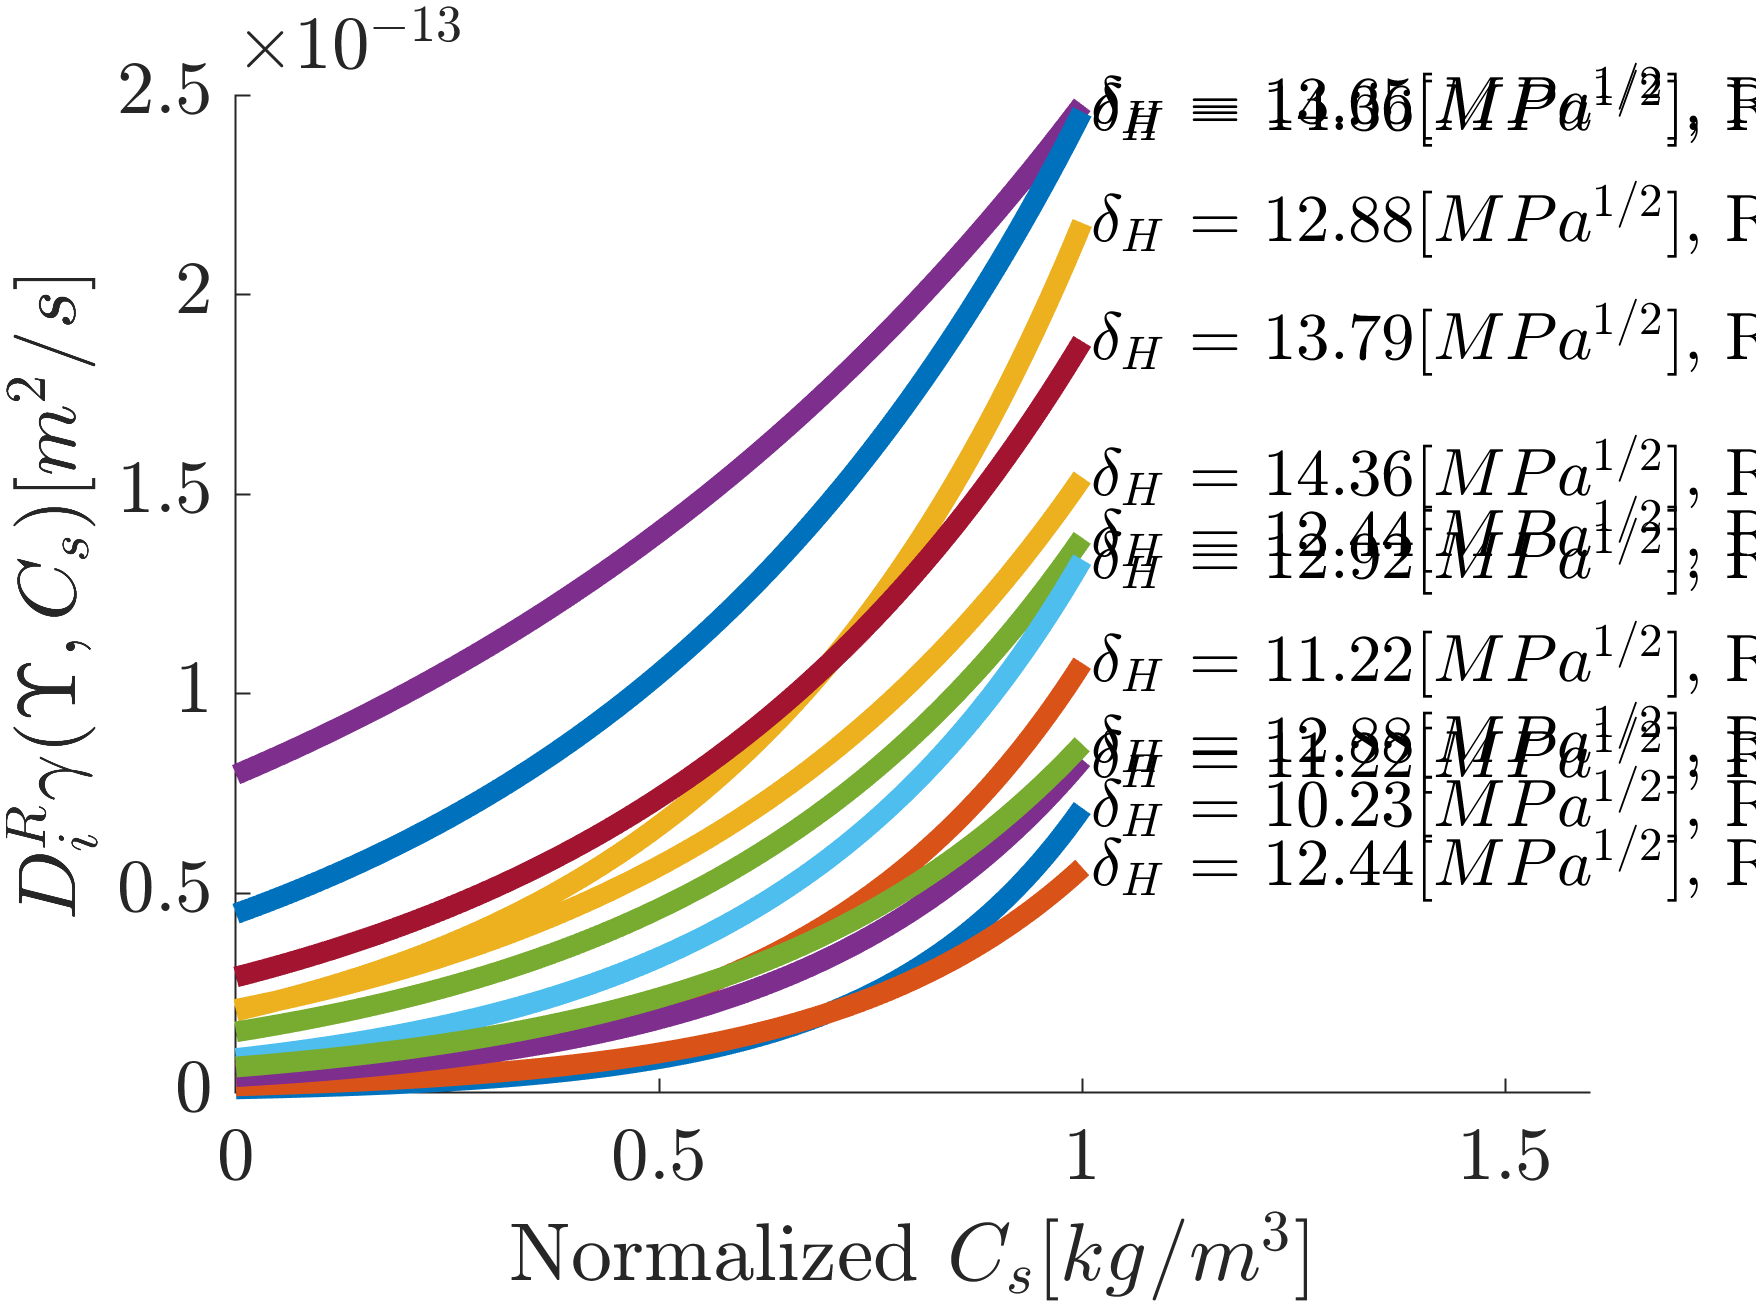
\includegraphics[trim = 0.0cm 0.0cm 0.0cm 0.0cm,clip, width=\columnwidth]{/Results_estimation/Gamma_function.png}
		\caption{The decaying internal diffusion coefficient}
		\label{fig: Gamma_function}
	\end{figure}
		
	The parameter estimation results are combined to analyse the relationship between the obtained parameters and the operating conditions. Unlike traditional methods that employ a combination of Reynolds, Schmidt, and Sherwood numbers to find correlations—omitted here due to the insignificance of axial diffusion—the approach in this study leverages the Reynolds number $\left(Re = \frac{(2r) \cdot \rho_f \cdot u}{\mu}\right)$ as the sole independent variable. Using the Reynolds number has the advantage of considering the influence of all the control variables (temperature, pressure and flow rate), which means it can be uniquely defined by selecting operating conditions.	
	
	In Figures \ref{fig: Correlations_Di_Re} and \ref{fig: Correlations_Gamma_Re}, two distinct data clusters emerge, each corresponding to a different mass flow rate. Despite the linear trends observed in both sets of correlations, the correlations for $D_i^R$ exhibit a decline with increasing Re, whereas those for $\Upsilon$ show an upward trend with Re. The decrease in $D_i^R$ across each data line can be attributed to higher fluid density and increased mass transfer resistance. Conversely, the rise in $\Upsilon$ correlations may be explained by enhanced solubility. The Hildebrand solubility factor and the Reynolds number are proportional to the fluid density; hence, $\Upsilon$ can be correlated with Re.
	
	\begin{figure}[!h]
		\centering
		\begin{subfigure}[b]{\columnwidth}
			\centering
			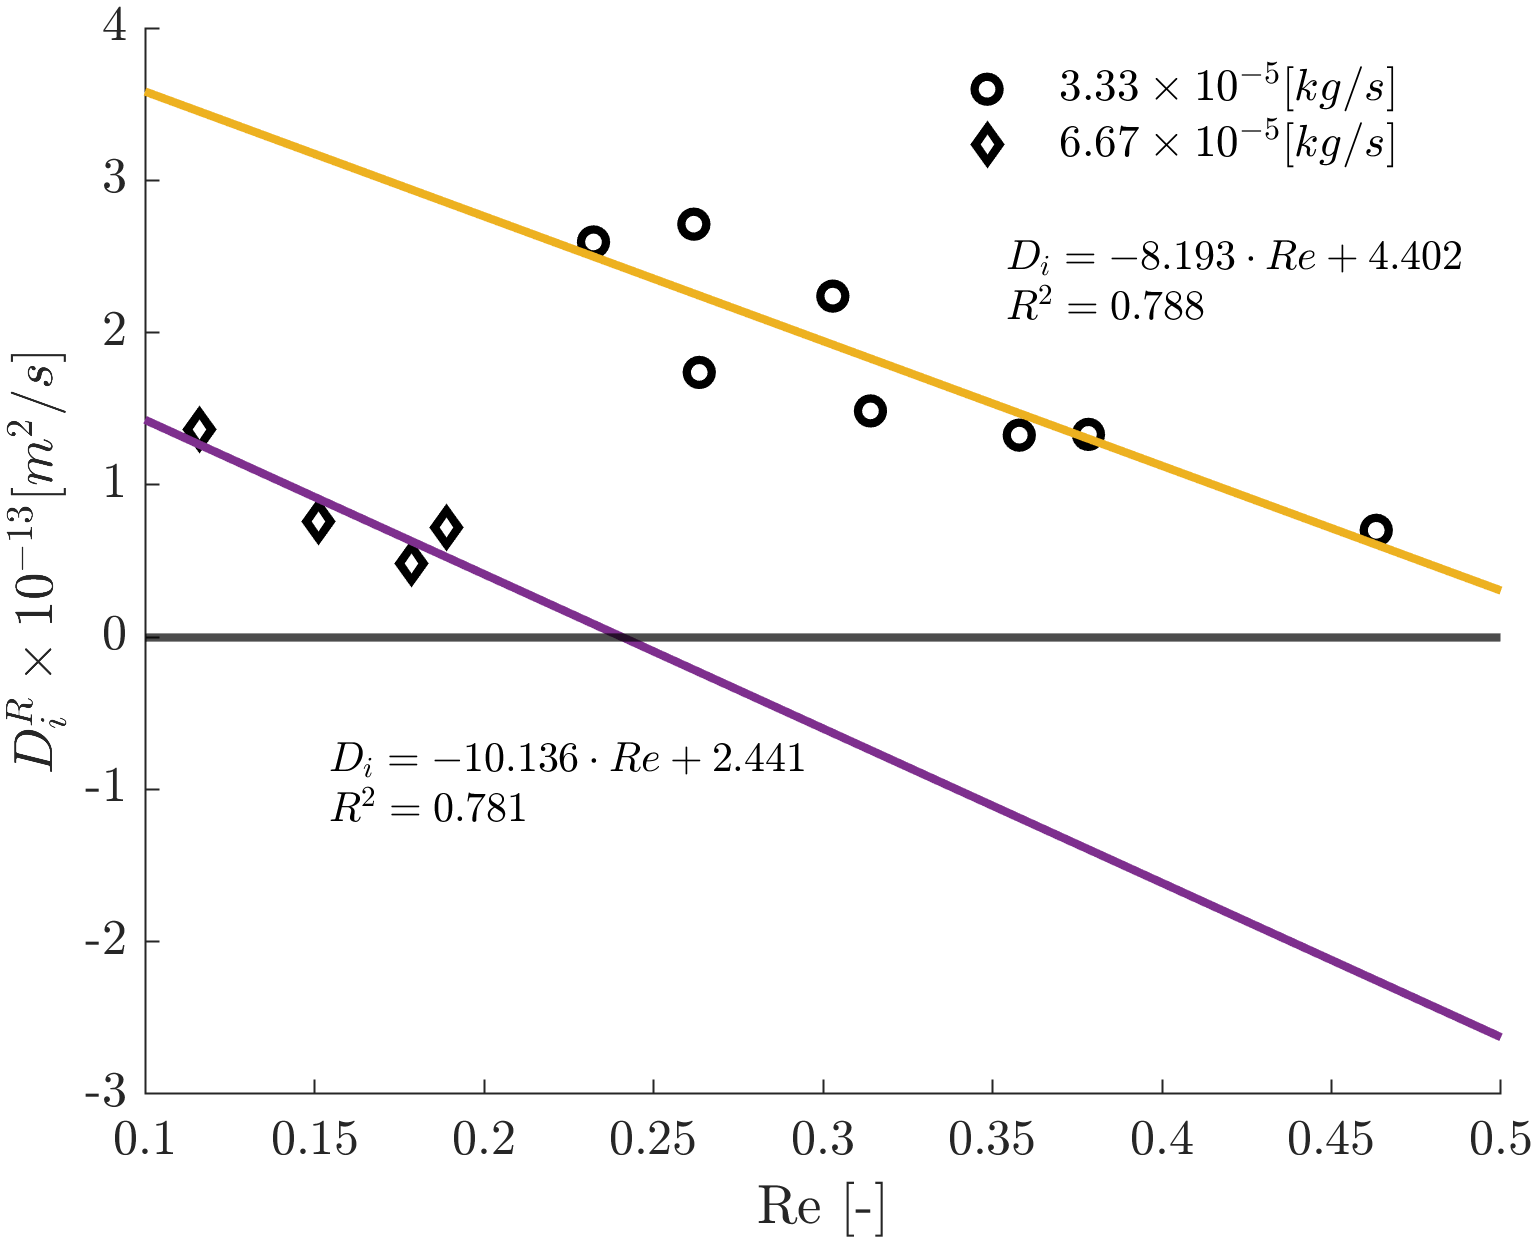
\includegraphics[trim = 0.0cm 0.0cm 0.0cm 0.0cm,clip, width=\columnwidth]{/Results_estimation/Correlation_Di_Re.png}
			\caption{Linear regression $D_i^R = f(Re)$}
			\label{fig: Correlations_Di_Re}
		\end{subfigure}
		\hfill
		\begin{subfigure}[b]{\columnwidth}
			\centering
			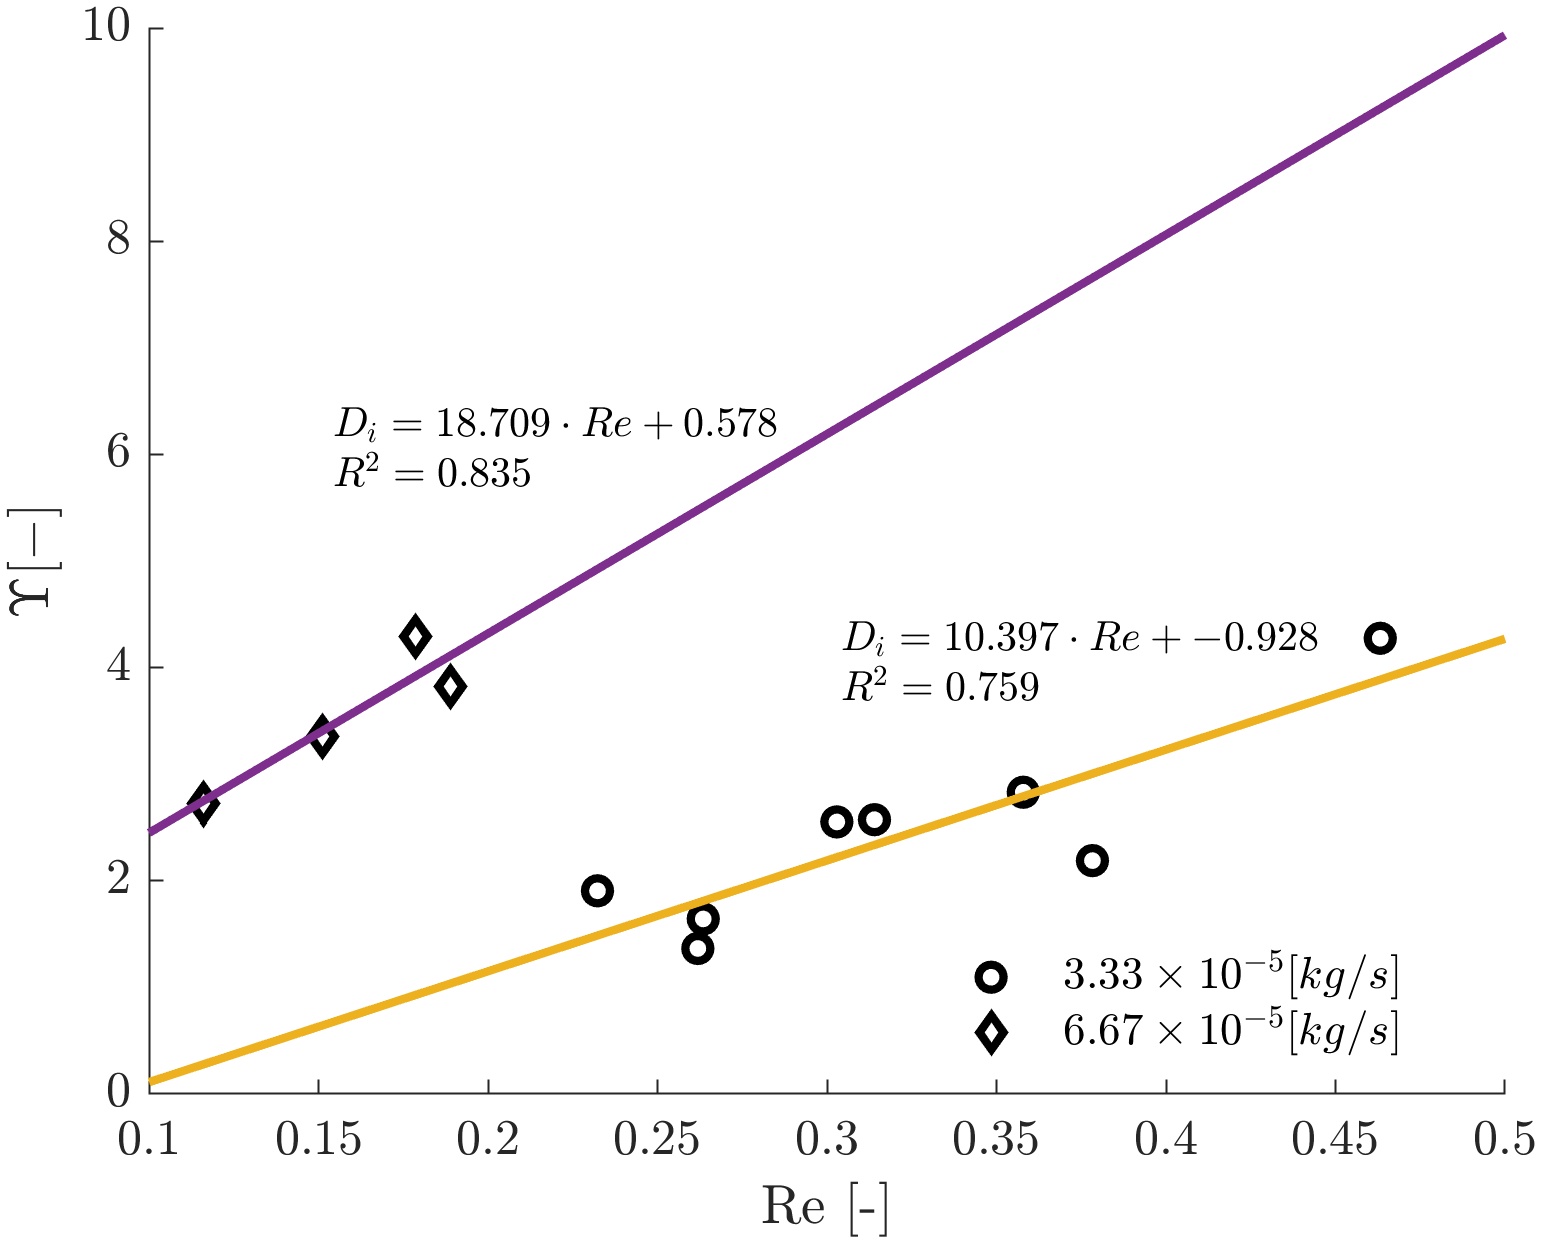
\includegraphics[trim = 0.0cm 0.0cm 0.0cm 0.0cm,clip, width=\columnwidth]{/Results_estimation/Correlation_Gamma_Re.png}
			\caption{Linear regression $\Upsilon = f(Re)$}
			\label{fig: Correlations_Gamma_Re}
		\end{subfigure}
		\caption{Parameter estimation results}
		\label{fig: Correlations}
	\end{figure}
	
	A more general relationship can be obtained by applying multiple linear regression instead of linear regression. The clusters in Figure \ref{fig: Correlations} are close to parallel, suggesting that a plane would combine all the data points. The Reynolds number and flow rate act as independent variables for $D_i^R$ and $\Upsilon$ as presented in Figure \ref{fig: Correlations_surface}.
	
	\begin{figure}[!h]
		\centering
		\begin{subfigure}[b]{\columnwidth}
			\centering
			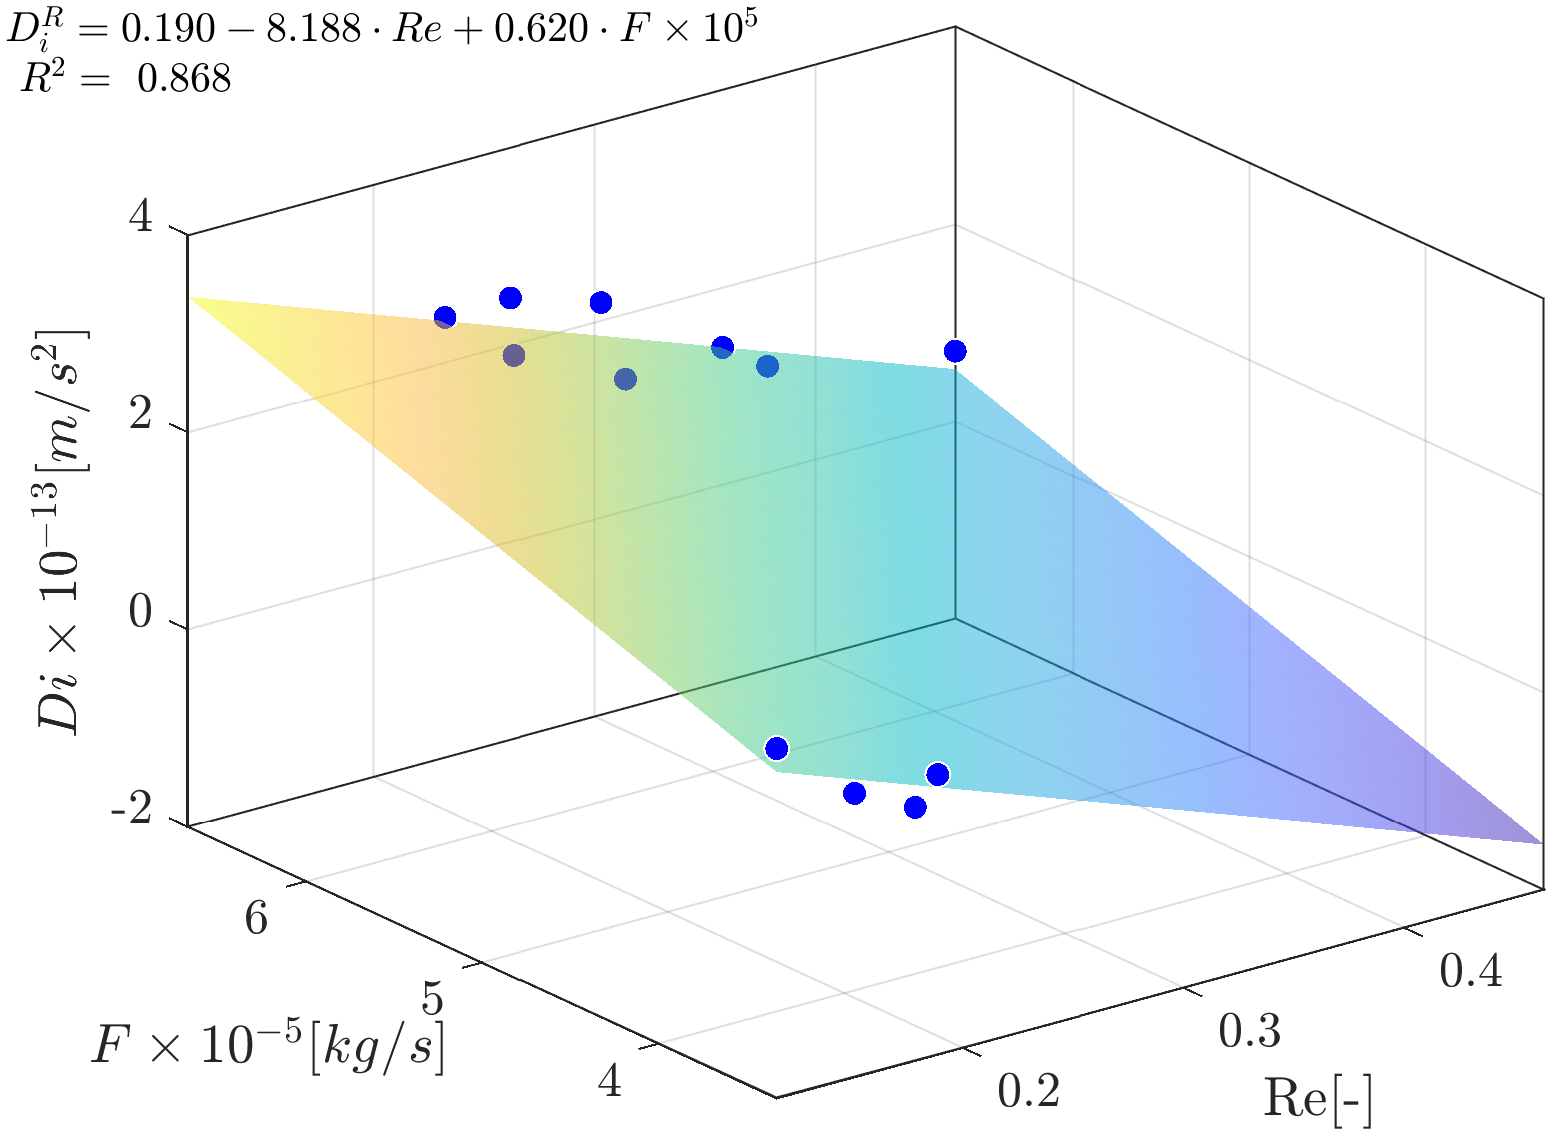
\includegraphics[trim = 0.0cm 0.0cm 0.0cm 0.0cm,clip, width=\columnwidth]{/Results_estimation/Di_Re_F.png}
			\caption{Multiple linear regression $D_i^R = f(Re, F)$}
			\label{fig: Correlations_Di_Re_F}
		\end{subfigure}
		\hfill
		\begin{subfigure}[b]{\columnwidth}
			\centering
			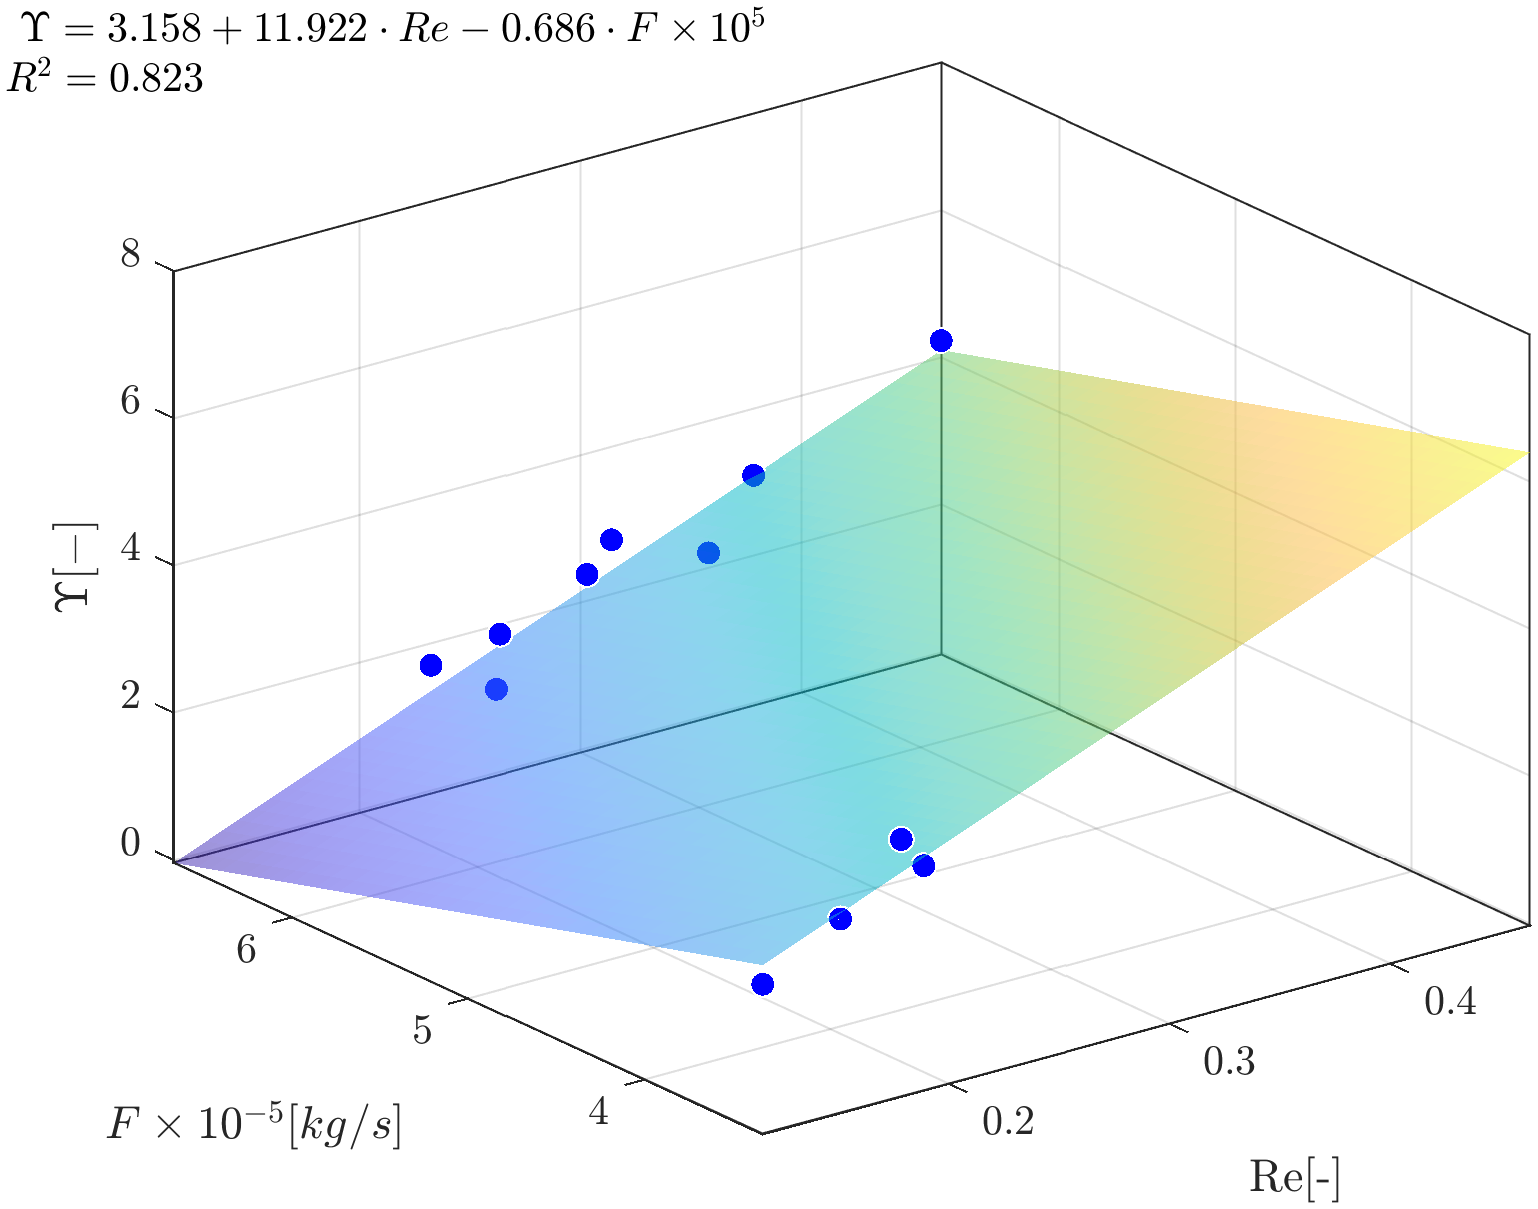
\includegraphics[trim = 0.0cm 0.0cm 0.0cm 0.0cm,clip, width=\columnwidth]{/Results_estimation/Gamma_Re_F.png}
			\caption{Multiple linear regression $\Upsilon = f(Re, F)$}
			\label{fig: Correlations_Gamma_Re_F}
		\end{subfigure}
		\caption{Parameter estimation results}
		\label{fig: Correlations_surface}
	\end{figure}
	
	
\end{document}